\section{Analysis}
\subsection{Functional Requirements and Use Cases}
\subsubsection{Use Cases List}
\begin{itemize}
	\item An \textit{unregistered user} can
	\begin{itemize}
		\item Register
	\end{itemize}
	\item A \textit{registered user} can
	\begin{itemize}
		\item Login
		\item Consult Pokèdex
		\begin{itemize}
			\item Search by Name
			\item Search by Type(s)
			\item Search by Pokédex ID
			\item Search by Catch Rate
			\item Search by Points  
			\item Search by Pokemon characteristics like Height or  Weight
		\end{itemize}
		\item Consult ranking:
		\begin{itemize}
			\item Most popular Pokèmon among all Users
			\item Most popular Pokèmon in each Country
			\item Best World Teams
			\item Best Teams among Friends
			\item Best Teams by Country
		\end{itemize}
		\item Find Users:
		\begin{itemize}
			\item See recommended users based on common friends
			\item See recommended users based on common Pokémon interests
			\item Find users by username
			\item Follow/Unfollow them
		\end{itemize}
		\item Interact with Pokèmon network:
		\begin{itemize}
			\item Insert/Remove a Pokémon in his/her own favorite Pokémon list
			\item Create a post on a Pokémon to share opinions
			\item Add answers to posts
			\item Follow/Unfollow them
			\item The post owner can also remove the post at his/her will
		\end{itemize}
		\item Team handling:
		\begin{itemize}
			\item Remove Pokemon from the team
			\item View team
			\item Change name of the Team	
			\item Save modified team
			\item View the value of the team
		\end{itemize}
		\item Catching:
		\begin{itemize}
			\item Browse a Pokémon you want to catch searching it by name 
			\item Select a Pokémon you want to catch from the list of favorites
			\item Try to catch a Pokemon to add to your Team
		\end{itemize}
		\item Settings:
		\begin{itemize}
			\item Change Email
			\item Change Password
			\item Change Country
		\end{itemize}
		\item Logout:
		\begin{itemize}
			\item Exit from the account
			\item Return to the sign in window
		\end{itemize}
		\item At each time can:
		\begin{itemize}
			\item See the remaining daily Pokèballs
			\item Mute/Unmute Music
			\item \colorbox{BurntOrange}{By clicking on a Pokémon name, visualize all the information about it} 
		\end{itemize}
	\end{itemize}
	\item An \textit{admin} can
	\begin{itemize}
		\item Sign In
		\item Add Pokèmon to the Pokédex
		\item Remove Pokèmon from the Pokédex
		\item See the number of registered Users in time
		\item See the numbers of login per day
		\item See the numbers of login per day in every Country
		\item Remove a User from the system
		\item Remove Posts/Answers from the system
		\item Consult Rankings
		\item Logout
\end{itemize}
	\item The \textit{system} should
	\begin{itemize}
		\item Daily update Pokeball number of each user
		\item Periodically update Pokemon catch rates based on the number of users that own that pokemon
		\item Update team points if the user has 6 Pokémon of different types
		\item Periodically compute usage statistics to be consulted by the administrators
	\end{itemize}
\end{itemize}

\subsubsection{UML Use Cases Diagram}
\begin{figure}[H]
	\centering
	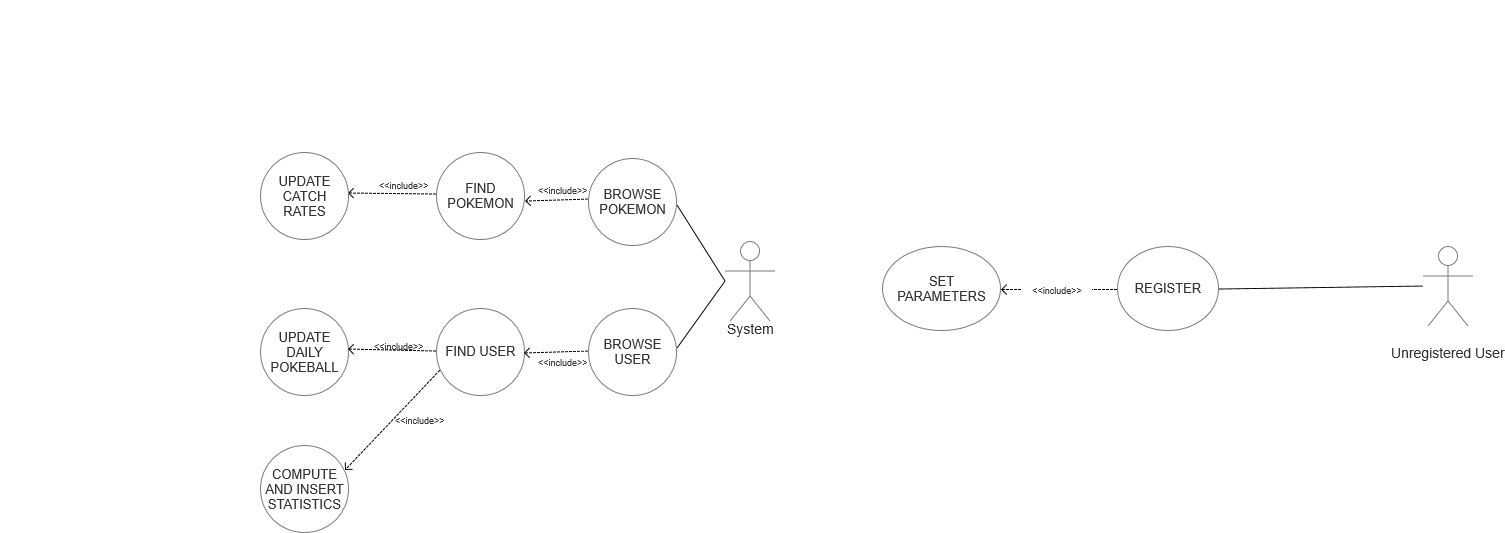
\includegraphics[width=\textwidth]{img/uml_use_case_2.png}
	\caption{Use Case Diagram 1}
\end{figure}
\begin{figure}[H]
	\centering
	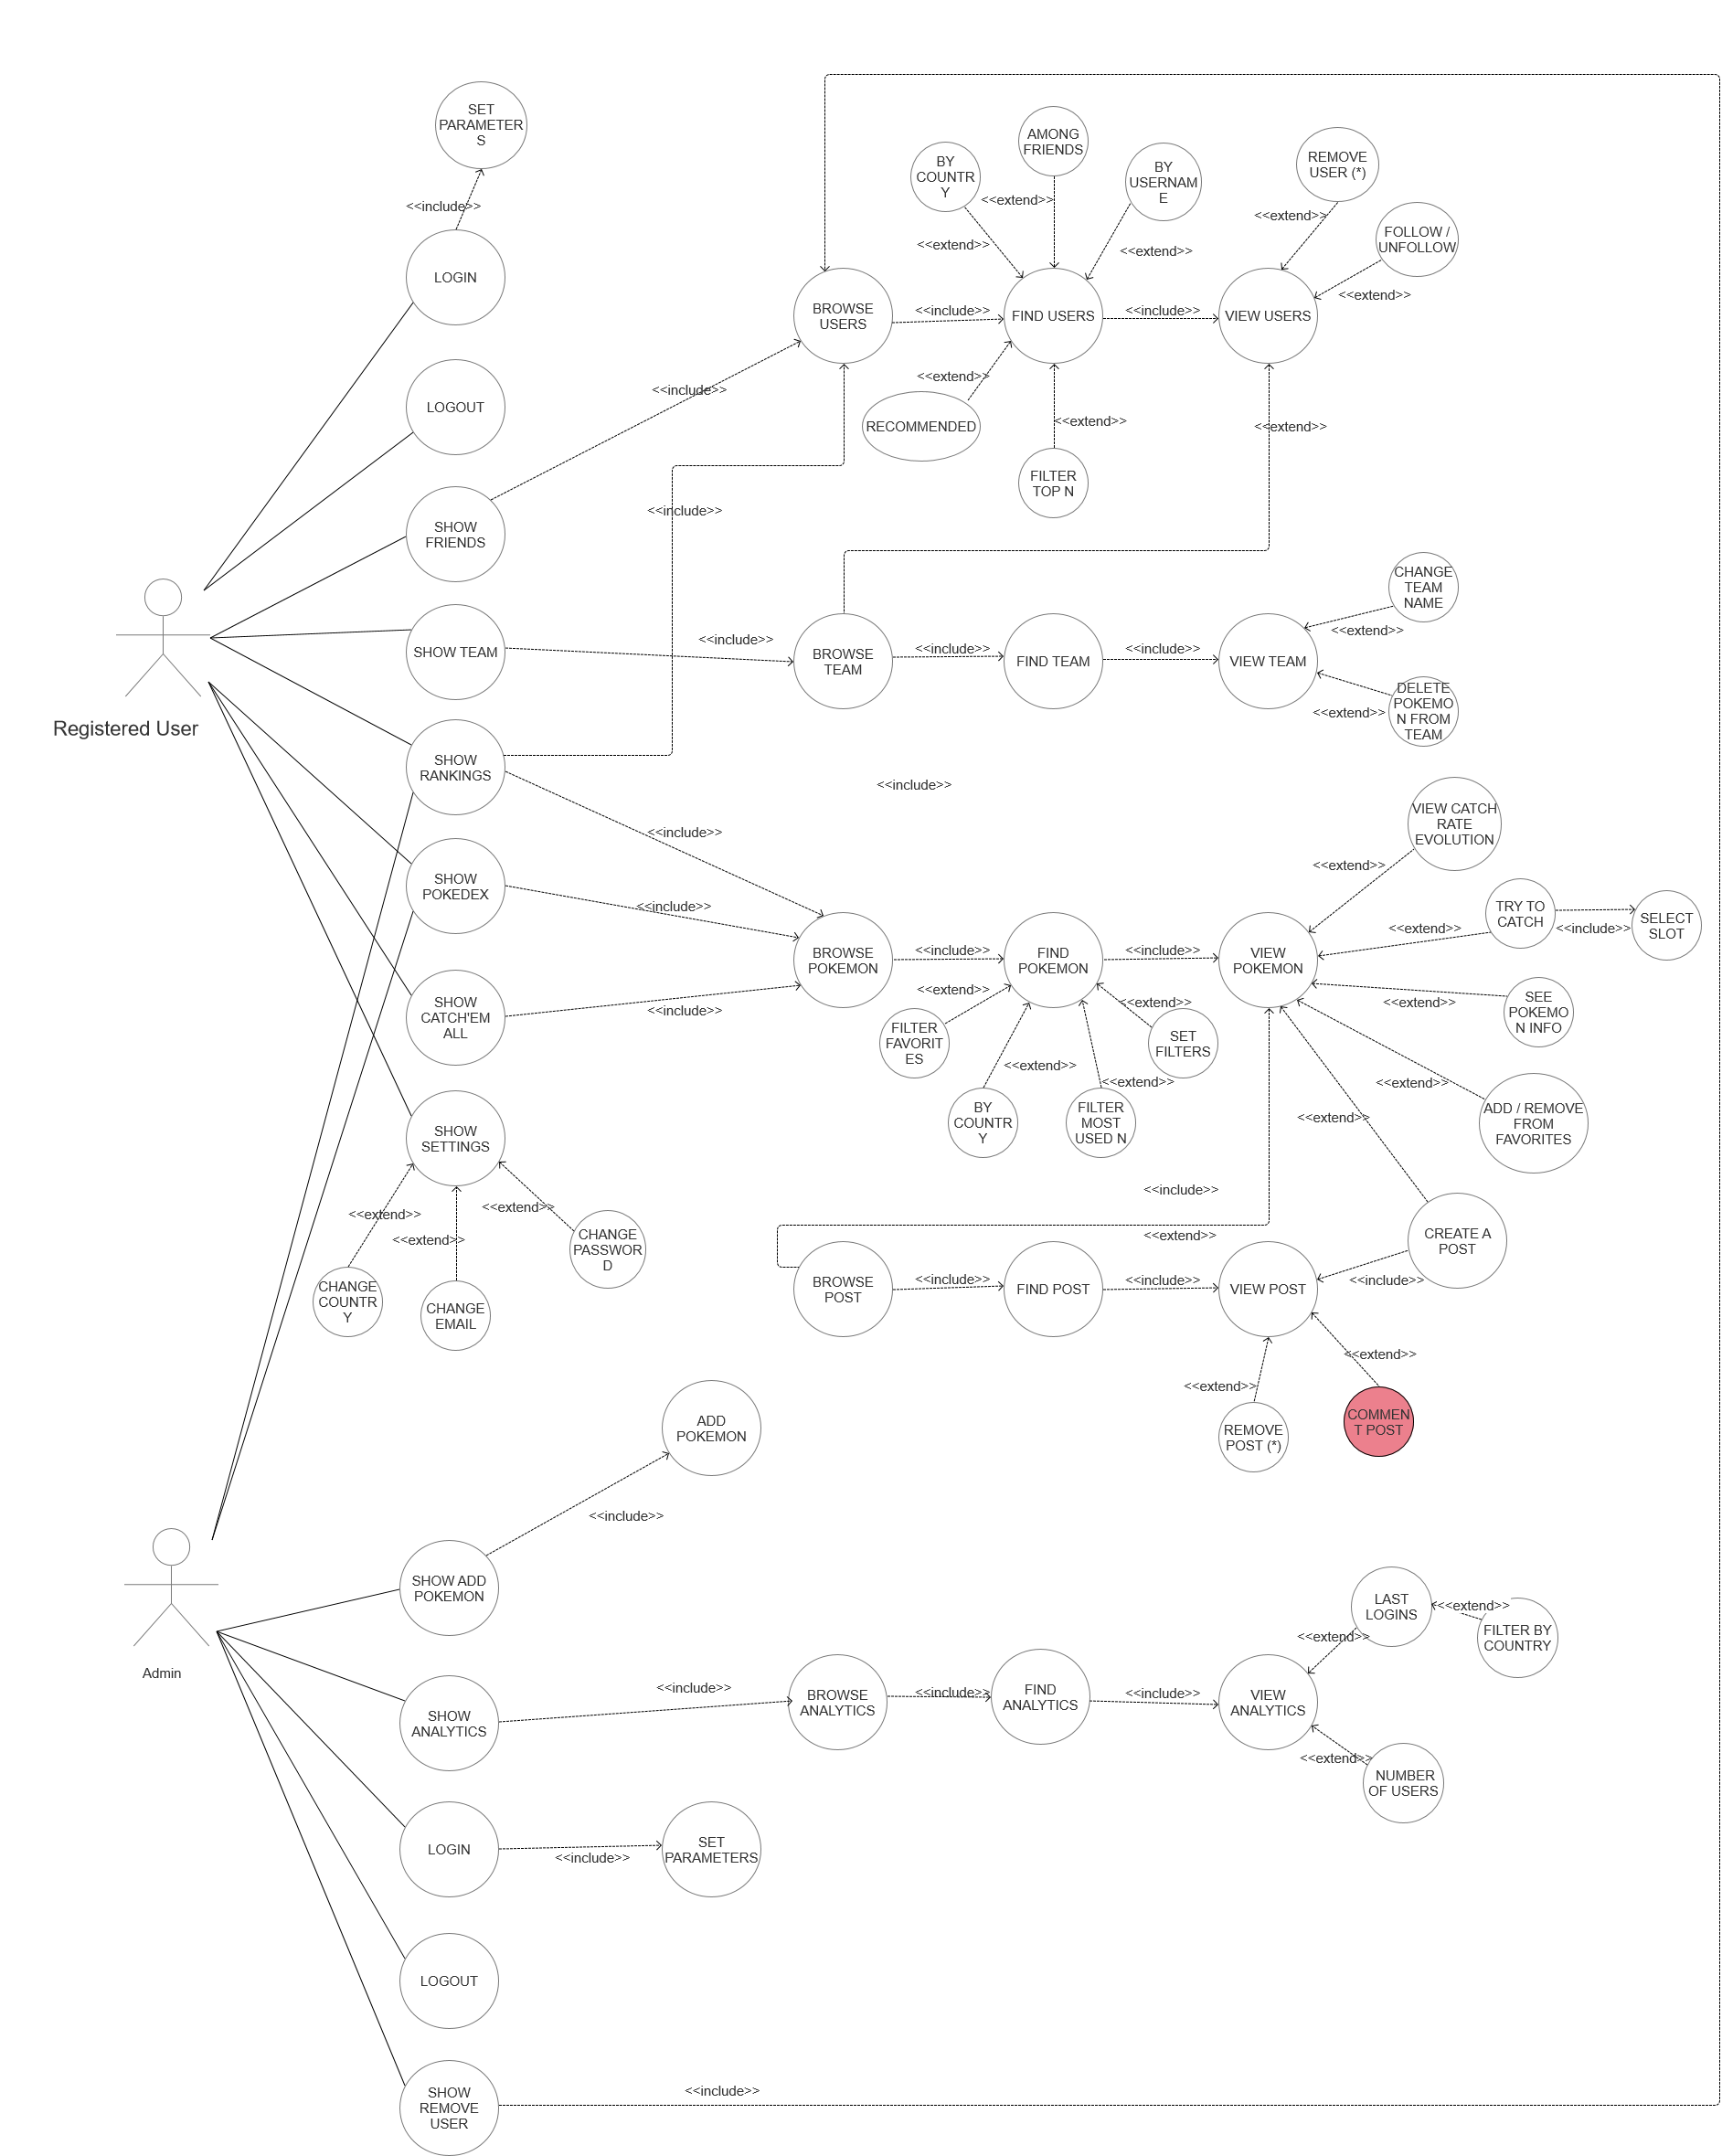
\includegraphics[width=\textwidth]{img/uml_use_case_1.png}
	\caption{Use Case Diagram 2\\ (*) only for the User who created the Post and Admins, in  \colorbox{Red}{Red} Browse-find-view comments and browse-find-view answers had not been reported )}
	
\end{figure}


\subsection{Non-Functional Requirements}
\begin{itemize}
	\item The application should guarantee a high availability. The application should guarantee a \textbf{high availability}
	\item It should be \textbf{easy to use}, especially for children and youngsters, and enjoyable
	\item It should have a \textbf{read-your-own-writes consistency} on each user’s own team, so he/she can always be sure that Pokémon have been correctly caught/freed up
	\item \colorbox{BurntOrange}{The application should always provide to each user} the most recent version of the rankings in order to permit him/her to immediately verify his/her progresses
	\item The statistics regarding usage and catch rate evolution are not needed to be real-time, they can be updated periodically and be eventually consistent
	\item Posts, comments and answers must follow a \textbf{causal-consistency}
	\item \textbf{Response time} is an important issue: redundancies and larger memory consumptions are preferred over high latencies
	\item \textbf{Passwords are crypted} for security reasons
	\item A graphical interface and the usage of multimedia are crucial for an involving game experience 
\end{itemize}
\subsection{Sources, Velocity properties and Volume of data}
Data stored in the application backend has been downloaded and imported from the following sources:
\begin{enumerate}
	\item \textbf{Pokèmon Data} $\rightarrow$ \url{https://pokeapi.co},\\ \url{https://bulbapedia.bulbagarden.net/wiki} 
	\item \textbf{Countries data} $\rightarrow$ \url{https://gist.github.com/kalinchernev/486393efcca01623b18d}
	\item \textbf{Data for the generation of realistic users} $\rightarrow$  \url{https://github.com/smashew/NameDatabases/blob/master/NamesDatabases/surnames/all.txt}
\end{enumerate}

All the imported data has been modified, updated and preprocessed in order to satisfy the application needs. 
Users added have the only purpose of showing the application functionalities, \textbf{for privacy issues they are not real people}; anyway they have been created using \textit{realistic criteria}. \medskip\\
\textbf{Velocity} is guaranteed by the dynamic catch rate mechanism: the popularity of a Pokémon influences both its catch rate and the amount of points that it will provide. As a consequence, Users are continuously stimulated by catching new Pokémon, in order to try to raise their amount of points: in this way old teams’ data becomes quickly out-of-date. \\
\textbf{Volume} of data, considering 250K users, almost 1K Pokémon and about 500K posts is no lower than 100Mb.\\
\subsection{UML Entities Diagram}
\begin{figure}[H]
	\centering
	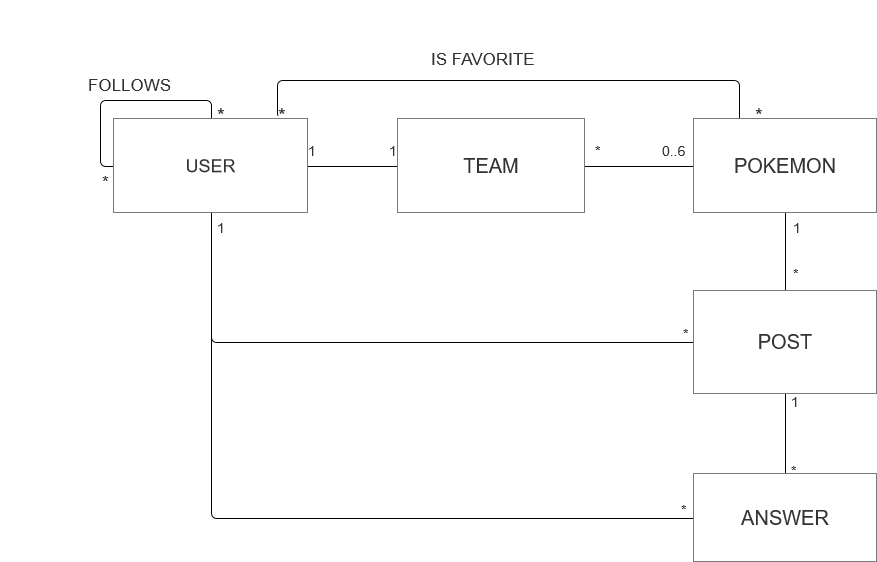
\includegraphics[width=\textwidth]{img/entity_diagram.png}
	\caption{UML Entity Diagram}
\end{figure}
\begin{enumerate}
	\item A \textbf{User} can build up only one \textbf{Team}: of course, each \textbf{Team} has just one owner.
	\item A \textbf{Team} is composed of a maximum of six \textbf{Pokémon}, every \textbf{Pokémon} can be caught by anyone, so can belong to many \textbf{Teams}.
	\item A \textbf{User} can follow many \textbf{Users}, in the meanwhile he/she can have many followers.
	\item A \textbf{User} can have many favorites \textbf{Pokémon}. A \textbf{Pokémon} can be favorite of many \textbf{Users}.
	\item A \textbf{Post} is created just by one \textbf{User} on one \textbf{Pokémon}. A \textbf{User} can create many posts and a \textbf{Pokémon} can have many \textbf{Posts} talking about it.
	\item An \textbf{Answer} is written by one \textbf{User} and it refers to one \textbf{Post}. \textbf{Users} can submit many Answers and there can be many \textbf{Answers} behind a \textbf{Post}.
\end{enumerate}
\subsection{Main application queries}
\begin{itemize}
	\item Insert a \textbf{User} into the system at registration time
	\item Create a new \textbf{Pokémon} (admin only)
	\item Insert a \textbf{Pokémon} into a \textbf{Team}
	\item Create a new \textbf{Post}
	\item Create a new \textbf{Answer}
	\item Create a follow relationship
	\item Add a \textbf{Pokémon} to the favorites
	\item Retrieve \textbf{User} information at login time
 	\item Retrieve a \textbf{User} by username when looking for a new friend
	\item Retrieve \textbf{Team} information based on user
	\item Retrieve \textbf{Pokémon} information using several filters
	\item Retrieve recommended \textbf{Users}
	\item Retrieve list of a \textbf{User}’s friends
	\item Retrieve a \textbf{Pokémon} by name when trying to catch it
	\item Retrieve all the \textbf{Posts} relative to a Pokémon
	\item Retrieve all the \textbf{Answers} to a \textbf{Post}
	\item Retrieve \textbf{User}’s favorite \textbf{Pokémon} 
	\item Modify \textbf{User} settings (email, password, country)
	\item Update \textbf{Team}’s name
	\item Update \textbf{Team}’s points
	\item Update \textbf{Pokémon}’s catch rates Analytics: find $\%$ of \textbf{Users} that own that \textbf{Pokémon}
	\item Remove a \textbf{User} (admin only)
	\item Remove a \textbf{Pokémon} (admin only)
	\item Remove a \textbf{Post} (only admin and post’s owner)
	\item Remove a follow relationship
	\item Remove a \textbf{Pokémon} from the favorite ones
	\item Analytics: ranking of most popular \textbf{Pokémon} in world/each country
	\item Analytics: ranking of best \textbf{Teams} in the world/each country/among friends
	\item Analytics: evolution on time of a \textbf{Pokémon} catch rate
	\item Analytics: evolution on time of number of logins per day/total \textbf{Users}/logins per day by country (admin only)
\end{itemize}